\section{Diskussion}
\label{sec:Diskussion}

Die Versuchsdurchführung verlief ohne größere Probleme.
Einge Messwerte mussten zweimal aufgenommen werden, da das Oszilloskop nicht alle Spannungsverläufe gespeichert hat.
Während der Versuchsdurchführung sind keine größeren Abweichungen aufgefallen, dennoch zeigt die Ausgleichsrechnung im Vergleich zu den notierten Werten starke Abweichungen.
Dies fällt besonders beim Durchlauf ohne Noise Generator auf.
Eine Art Übereinstimmung fällt bei der Abzisse auf, für $\phi = 0 , 180 und 360$ befinden sich Extrema.
Trotzdem wirken die Messergebnisse nicht zur Ausgleichskurve passend.
Im Diagramm mit dem Noise Generator liegen die größten Spannungen auch in der Nähe der Maxima des Fits, andere Werte liegen fast genau auf dem Graphen.

\noindent
Für die Eingangsspannungen wurden folgende Werte ermittelt:
\begin{align*}
    \text{ohne Noise Generator:}&  &U_0_\text{ohne} &= \SI{26.70 \pm 16.80}{\volt}, \\
    \text{mit Noise Generator:}&   &U_0_\text{mit}  &= \SI{ 6.28 \pm 4.56}{\volt}.
\end{align*}

EIGENTLICHE EINGANGSSPANNUNG? 10 MV? 

\noindent
Bei der Untersuchung mithilfe der Photodioden müssen die Lichtverhältnisse berücksichtigt werden.
Die Deckenlampen wurden alle ausgeschaltet, dennoch kam genug Licht durch die Fenster hinein.
An diesen Umständen konnte nichts weiter geändert werden und hätte den Versuch stark beeinflussen können.
Die Messwerte zeigen aber gute Ergebnisse.
Die gewünschte $\sfrac{1}{r}$ Abhängigkeit ist gut zu sehen.
Da aber der Versuchsaufbau seine Grenzen hat und die Lichtverhältnisse auch nicht zu vernachlässigen sind,
konnte kein Extremwert aufgenommen werden, bei der die zu aufnehmende Spannung gegen Null geht.
Als maximaler Abstand und minimale Spannung wird somit $r = \SI{100}{\centimetre}$ und $U = \SI{126}{\volt}$ aufgenommen.

\section{Anhang}
\begin{figure}
    \centering
    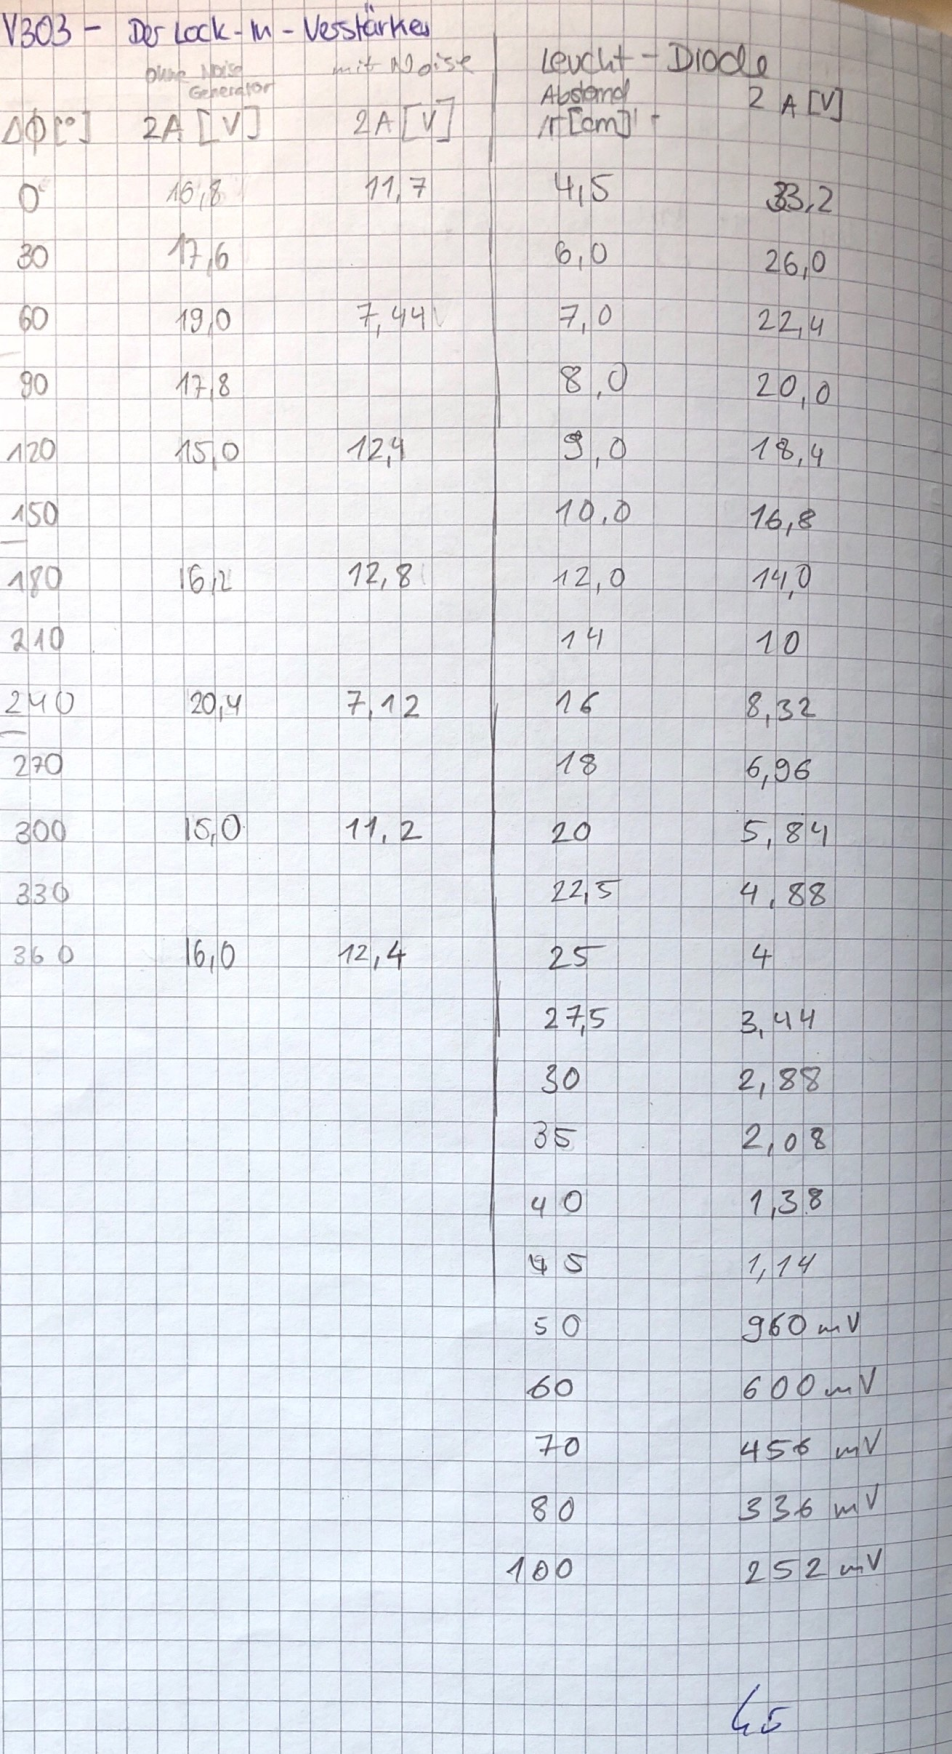
\includegraphics[width=\textwidth]{bilder/data_v303.pdf.pdf}
    \caption{Die Originaldaten von der Versuchsdurchführung.}
\end{figure}